\documentclass{article}

\usepackage{tikz}
\usetikzlibrary{automata, quotes, calc, arrows.meta}
\usepackage[czech]{babel} 
\usepackage[utf8]{inputenc}
\usepackage[T1]{fontenc}
%\usepackage[IL2]{fontenc} % Different type of font for wierdos
\usepackage{graphicx} % Required for the inclusion of images
\usepackage{natbib} % Required to change bibliography style to APA
\usepackage{amsmath} % Required for some math elements 
\usepackage{amsfonts}
\usepackage{amssymb}
\usepackage{booktabs}
\usepackage{epstopdf}
\usepackage{multicol}
\usepackage{color}
\usepackage{float}
\usepackage[total={15.5cm,23.5cm}, top=2.5cm, left=3cm, includefoot]{geometry}
\usepackage[colorlinks=true,linkcolor = black, urlcolor = black, citecolor = black]{hyperref}
\usepackage{enumitem}
\usepackage{subfig}
\usepackage[toc,page]{appendix}
\usepackage{hyperref} 
\usepackage{Matlab-prettifier}
\usepackage{datetime}
\usepackage{mathtools}
\usepackage[thinc]{esdiff}
\usepackage{listings}
\usepackage{xcolor} % For custom colors

\begin{document}


\begin{titlepage}

\centering

{\scshape\LARGE Západočeská univerzita\par}
{\scshape\Large Fakulta aplikovaných věd \par}
{\scshape\Large Katerdra Kybernetiky \par}
{\begin{center}
    
\includegraphics[width=0.7\textwidth]{pic/fav.jpg} 
\end{center}}

{\huge\bfseries První semestrální práce z STP \par}

\vspace{2cm}

{\Large\itshape Samuel Kokoška, Martin Hamar\par}

\vfill

\vspace{1cm}

\hskip -1 cm{KKY/STP} \hfill {Datum: \today }



\end{titlepage}

\section{Úvod}
V rámci první semestrální práce ze předmětu `Stochastické systémy a procesy' je cílem vypracovat dva příklady týkající se Markovských řetězců.
V prvním příkladu musí být řetězec regulární a homogenní a máme pro něj určit střední počet kroků, které jsou třeba k prvnímu dosažení stavu \verb|j| za předpokladu, že se vycházelo ze stavu \verb|i|. Poté máme také určit finální pravděpodobnosti.

V druhém příkladu pracujeme s homogenním řetězecem, kde jsou dva absorpční stavy. 
Zde máme určit střední počet průchodů stavem \verb|j|, pokud se vychází ze stavu \verb|i|, do té doby než dojde k pohlcení. Poté musíme vypočítat dobu pobytu v každém tranzientním stavu. Poslední podúkol příkladu 2 je spočtení ppsti skončení v absorpčím stavu, pro všechny tranzientní stavy.
Celé zadání je k vidění v sekci~\ref{ssec:zadani}. 


Během vypracovávání byl použit Matlab pro jeho schopnost pracování s maticemi a rovnicemi. Postupy řešení pro jednotlivé příklady jsou k vidění v sekci \ref{sec:postup}.




\subsection{Zadání}\label{ssec:zadani}
\begin{figure} [htb!]
    \centering
    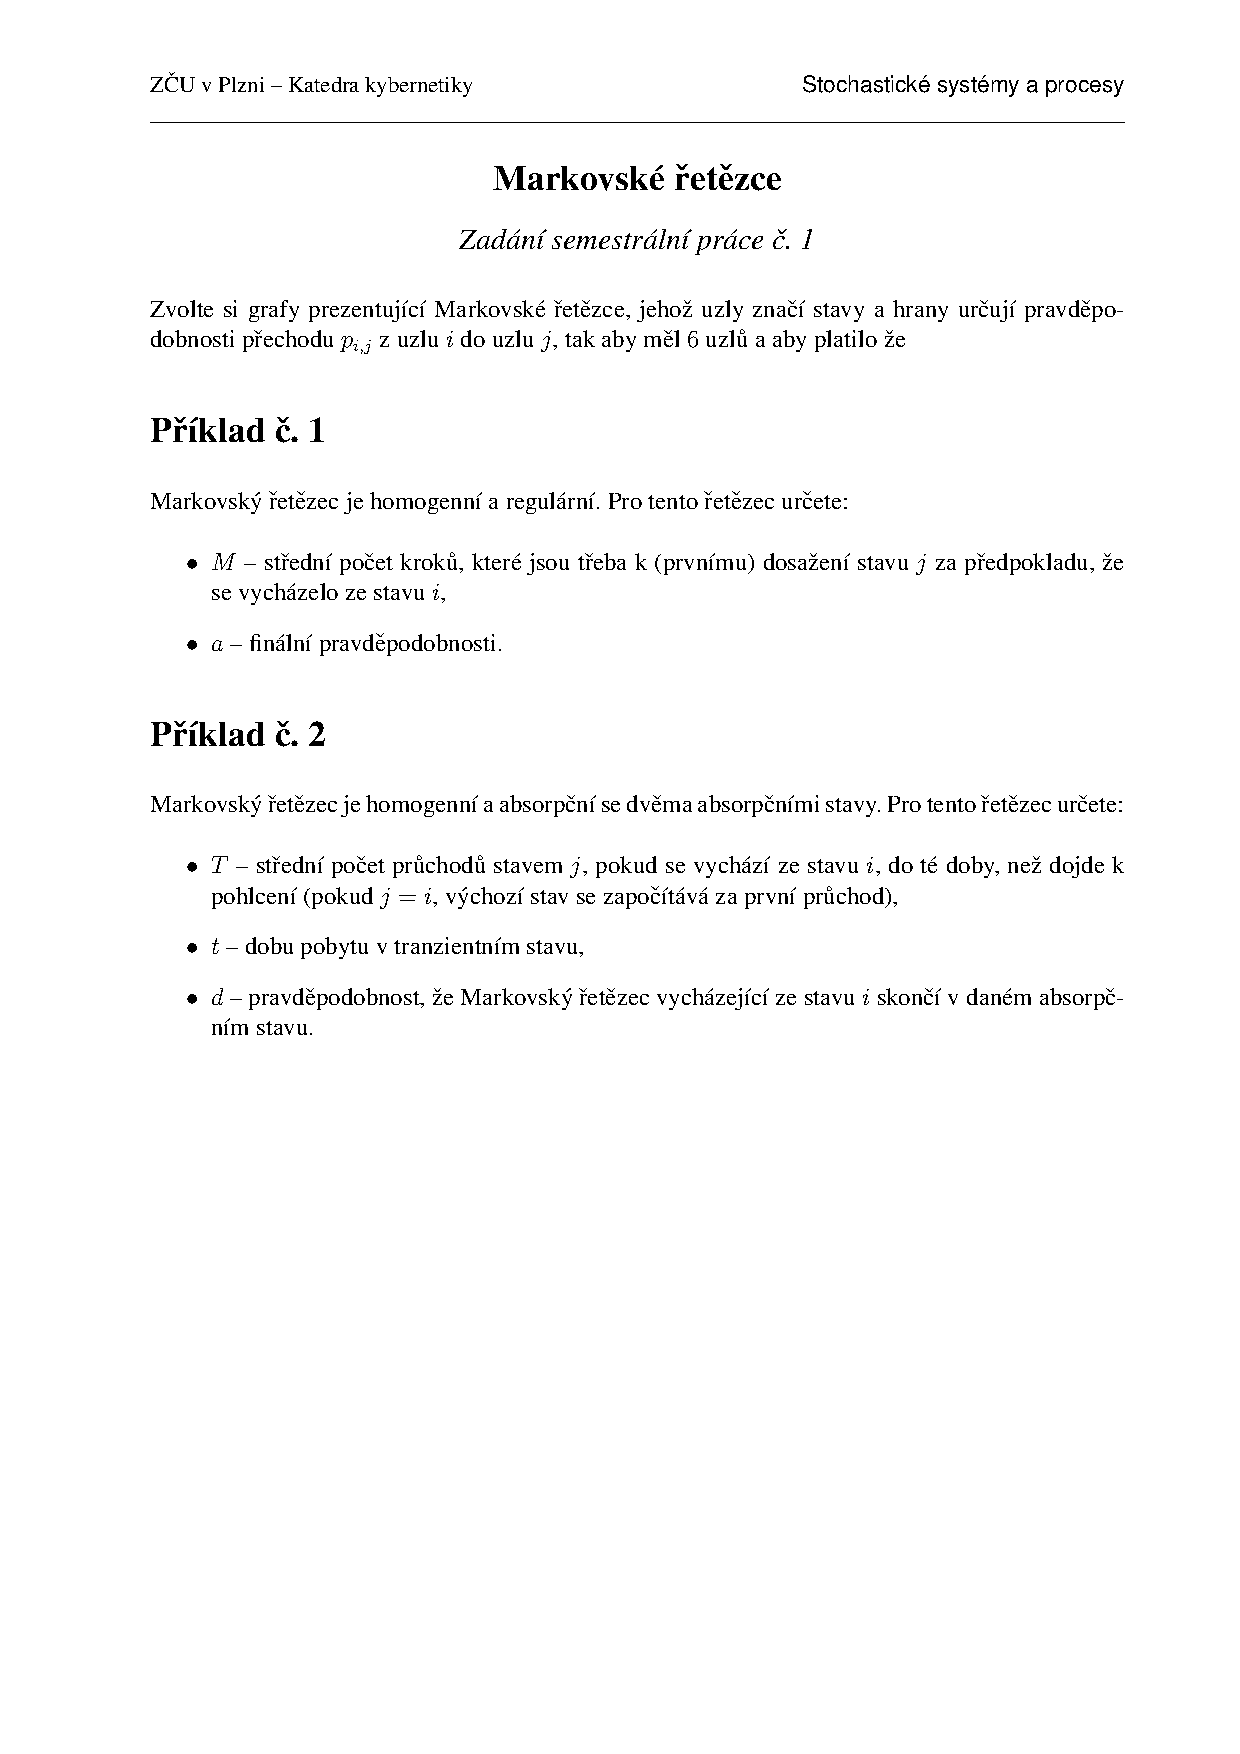
\includegraphics[width = 0.7\textwidth]{zadani.pdf}
    %\includesvg[width = 1\textwidth]{pic/XXX}
\end{figure}
\clearpage
\section{Postup Řešení}\label{sec:postup}
\subsection{Příklad 1}
Pro tento příklad by zvolen řetězec znázorněn na obrázku~\ref{fig:markov_chain_1}. Odpovídající matice $\mathbf{P}$ vypadá takto: 
\[
\mathbf{P} =
\begin{bmatrix}
0 & 0 & 1 & 0 & 0 & 0 \\
\addlinespace[3pt]
1 & 0 & 0 & 0 & 0 & 0 \\
\addlinespace[3pt]
0 & \frac{1}{2} & 0 & \frac{1}{2} & 0 & 0 \\
\addlinespace[3pt]
0 & 0 & \frac{1}{2} & 0 & \frac{1}{2} & 0 \\
\addlinespace[3pt]
0 & 0 & 0 & 0 & 0 & 1 \\
\addlinespace[3pt]
0 & 0 & 0 & 1 & 0 & 0 \\
\end{bmatrix}.
\]

U tohoto příkladu je snažší nejdříve spočítat finální ppsti.  Ty si spočítáme pomocí vztahu $\pi = \pi \mathbf{P}$, kde $\pi$ je vektor, který hledáme. Po úpravě řešíme soustavu rovnic: $(\mathbf{P}^T - \mathbf{I})\pi^T = \mathbf{0}$, za podmínky že členy vektoru $\pi$ mají součet jedna.
S vyřešením této rovnice nám pomůže Matlab a jejím výsledkem pro matici $\mathbf P$ sepsanou výše je:
\[
\pi = 
\begin{bmatrix}
    \frac 1 8 & \frac 1 8 & \frac 1 4 & \frac 1 4 &  \frac 1 8 & \frac 1 8 
\end{bmatrix}.
\]

Nyní si spočítáme matici $\mathbf{M}$, která určuje stření počet kroků, které jsou třeba k prvnímu dosažení stavu \verb|j| za předpokladu, že se vycházelo ze stavu \verb|i|. 
Zde na to půjdeme přes simulaci absorpčních stavů. 
Postupně uděláme z každého stavu absorpční a spočítáme pro něj fundamentální matici\footnote{Tento postup je využit i u příkladu 2, kde je vysvětlen podrobněji.} $\mathbf{T} = (\mathbf{I} - \mathbf{Q})^{-1}$.
Z té poté spočítáme střední dobu strávenou v tranzientních stavech $t = \mathbf{T}\mathbf{1}$ - to jsou všechny ty co nejsou absorpční. 
Tento vektor poté vložíme do matice $\mathbf{M}$, na místo určené vybraným absorpčním stavem. 

Je důležité podotknout, že tímto postupem získáme na diagonále nulové prvky, protože u tohoto výpočtu vždy považujeme daný diagonální prvek za absorpční a nemá smysl pro něj spočítat první dosažení.
Tyto diagonální prvky musíme spočítat pomocí následující rovnice: $m_{i,i}=\frac{1}{\pi_i}$, kde $m_{i,i}$ představuje prvek matice $\mathbf{M}$ na pozici $i,i$. Prvek $\pi_i$ představuje $i$-tý prvek vektoru $\pi$, vypočítaný v předchozím kroku.

Opět zde využijeme síly Matlabu a matice $\mathbf{M}$ nám vyjde následovně:
\[
    \mathbf{M} = 
\begin{bmatrix}
8 & 7 & 1 & 5 & 11 & 12 \\
1 & 8 & 2 & 6 & 12 & 13 \\
7 & 6 & 4 & 4 & 10 & 11 \\
11 & 10 & 4 & 4 & 6 & 7 \\
13 & 12 & 6 & 2 & 8 & 1 \\
12 & 11 & 5 & 1 & 7 & 8 \\
\end{bmatrix}.
\]

\shorthandoff{"}
\begin{figure}
\centering
\begin{tikzpicture}[%
    every edge/.style = {draw, -Stealth},
    every edge quotes/.append style = {auto, inner sep=2pt, font=\footnotesize}
]
\foreach \x in {1,...,6} {
    \node (s\x) [state] at (180-60*\x:3cm) {$s_\x$};
}
\path
    (s1) edge ["$1$", bend right=15] (s3)
    (s2) edge ["$1$", bend right=15] (s1)
    (s3) edge ["$\frac{1}{2}$", bend right=15] (s2)
        edge ["$\frac{1}{2}$", bend left=15] (s4)
    (s4) edge ["$\frac{1}{2}$", bend left=15] (s3)
        edge ["$\frac{1}{2}$", bend left=15] (s5)
    (s5) edge ["$1$", bend left=15] (s6)
    (s6) edge ["$1$", bend left=15] (s4)
        % (s4) edge ["$1$", loop right] (s4)

    ;
\end{tikzpicture}
\caption{Regulární Markovský řetězec}
\label{fig:markov_chain_1}
    
\end{figure}
\clearpage

\subsection{Příklad 2}
Pro příklad vezmeme podobný řetězec jako v prvním příkladu, ale ze stavů $s_1$ a $s_6$ uděláme absorpční - znázorněno na obrázku~\ref{fig:markov_chain_2}.
Tomuto řetězci odpovídá následující matice $\mathbf{P}$:
\[
\mathbf{P} =
\begin{bmatrix}
1 & 0 & 0 & 0 & 0 & 0 \\
\addlinespace[3pt]
1 & 0 & 0 & 0 & 0 & 0 \\
\addlinespace[3pt]
0 & \frac{1}{2} & 0 & \frac{1}{2} & 0 & 0 \\
\addlinespace[3pt]
0 & 0 & \frac{1}{2} & 0 & \frac{1}{2} & 0 \\
\addlinespace[3pt]
0 & 0 & 0 & 0 & 0 & 1 \\
\addlinespace[3pt]
0 & 0 & 0 & 0 & 0 & 1 \\
\end{bmatrix}.
\]

Pro splnění prvního podúkolu hledáme fundamentální matici $\mathbf{T}$. Tu nalezneme pomocí rovnice: $\mathbf{T}=(\mathbf{I}-\mathbf{Q})^{-1}$. Matice $\mathbf{Q}$ zde odpovídá matici $\mathbf{P}$, kde je vynechaný první a poslední řádek i sloupec (ty totiž odpovídají absorpčním stavům).
K odečtení jednotkové diagonální matice $\mathbf{I}$ a spočtení inverze opět použijeme Matlab a získáme následující matici $\mathbf{T}$:



\[
\mathbf{T} =
\begin{bmatrix}
1 & 0 & 0 & 0 \\
\addlinespace[3pt]
\frac{2}{3} & \frac{4}{3} & \frac{2}{3} & \frac{1}{3} \\
\addlinespace[3pt]
\frac{1}{3} & \frac{2}{3} & \frac{4}{3} & \frac{2}{3} \\
\addlinespace[3pt]
0 & 0 & 0 & 1 \\
\end{bmatrix}.
\]

Střední dobu strávenou v tranzietních stavech $t$ získáme sečtením hodnot jednotlivých řádků - tedy vynásobení matice $\mathbf{T}$ vektorem jedniček $\mathbf{1} = [1, 1, 1, 1]^T$.
\[
t = 
\begin{bmatrix}
    1 & 3 & 3 & 1
\end{bmatrix}^T.
\]

Nyní si musíme spočítat pravděpodobnost pohlcení pro oba absorpční stavy, začínáme-li ve stavu \verb|i|.
Pro oba stavy budeme řešit následující rovnici: $d = \mathbf{P} d$, kde vektor $d$, který má vždy pro jeden absorpční stav hodnotu $1$ a pro ostatní absorpční stavy $0$. 
Pro absorpční stav $s_1$ tedy je:\linebreak  $d~=~[1, d_2, d_3, d_4, d_5, 0]^T$, kde $d_2, d_3, d_4, d_5$ jsou prvky co hledáme. Pro stav $s_6$ je vektor velice podobný, má prohozenou ovšem jedničku s nulou.
K vyřešení obou rovnic (jedna rovnice odpovídá jednomu absorpčnímu stavu) byl využit \verb|syms| toolbox Matlabu.

Pro absorpční stav $s_1$ nám vyšel vektor $d$:
\[
d = 
\begin{bmatrix}
    1 & 1 &\frac 2 3 & \frac 1 3 & 0 & 0
\end{bmatrix}^T.
\]

A pro stav $s_6$ nám vyšel vektor $d$:
\[
d = 
\begin{bmatrix}
    0 & 0 & \frac 1 3 & \frac 2 3 & 1 & 1
\end{bmatrix}^T.
\]


\shorthandoff{"}
\begin{figure}
\centering
\begin{tikzpicture}[%
    every edge/.style = {draw, -Stealth},
    every edge quotes/.append style = {auto, inner sep=2pt, font=\footnotesize}
]
\foreach \x in {1,...,6} {
    \node (s\x) [state] at (180-60*\x:3cm) {$s_\x$};
}
\path
    (s1) edge ["$1$", loop left] (s1)
    (s2) edge ["$1$", bend right=15] (s1)
    (s3) edge ["$\frac{1}{2}$", bend right=15] (s2)
        edge ["$\frac{1}{2}$", bend left=15] (s4)
    (s4) edge ["$\frac{1}{2}$", bend left=15] (s3)
        edge ["$\frac{1}{2}$", bend left=15] (s5)
    (s5) edge ["$1$", bend left=15] (s6)
    (s6) edge ["$1$", loop right] (s4)
        % (s4) edge ["$1$", loop right] (s4)

    ;
\end{tikzpicture}
\caption{Markovský řetězec s dvěma absorpčními stavy}
\label{fig:markov_chain_2}
\end{figure}
\clearpage
\section{Závěr}
Cílem této práce bylo naučit se základní úlohy týkající se Markovských řetězeců. Pracovali jsme jak s regulárními řetězci, tak s řetězecem obsahující absorpční stav. 
Práce byla vypracována v Matlabu a napsáním tohoto referátu ji považuji za úspěšně splněnou.
\end{document}

